%Formatting Guidelines for Writing Dissertation.
\chapter{Introduction}\label{Guidelines}
A treatise advancing a new point of view resulting from research is one of the compulsory requirements of an academic degree of NIT Rourkela. Undergraduate\index{undergraduate} students submit a project report in support of their candidature for B.Tech. degree. Similarly, Masters\index{masters} students submit theses, and doctoral\index{doctoral} students submit dissertations. Unless otherwise stated explicitly, henceforth in this document the word ``dissertation'' will be used as a synonym for ``report'' and ``thesis''. 
\par This document is intended to provide a guideline to students in the preparation of their dissertations. A dissertation is expected to have ethical standards and uniform format with readability. NITR will accept dissertation only in pdf format, which should be uploaded directly to the NITR dissertation submission web page for approval by supervisor. Templates\index{template} to assist in formatting\index{formatting} dissertation in \LaTeX~ is available in \texttt{Academic -> Dissertation Template} at the URL \texttt{http://nitris.nitrkl.ac.in}.
\section{Dissertation Arrangement}
Each dissertation must be arranged in the following serial order. Optional pages may not be included.
\begin{itemize}
\item[i.] \textbf{Cover Page}\index{cover page}\\
The cover page comprises the dissertation title, author's name, and institutional details. This page is excluded from page number counter. A sample cover page design and spine design is shown in Figure~\ref{fig-Ch1-CoverPage}.
\begin{figure}[bh!]
\centering
	\begin{tikzpicture}[scale=1.3]
%			\draw[step=.5cm,red,very thin] (0,1) grid (12,19);
%			\draw[step=1cm,red,thick] (-1,1) grid (12,19);

			\draw[-,ultra thick](1,1)--(10.5,1)--(10.5,15)--(1,15);
			\draw[-,ultra thick](1,1)--(-.5,1);
			\draw[-,ultra thick](-.5,15)--(1,15);
			\draw[dashed, ultra thick](1,1)--(1,15);
			\draw[dashed, ultra thick](-.5,1)--(-.5,15);
			\node[font=\Large,right]at(1.5,13){\textbf{Guidelines for Formatting Dissertation}};
			\node[font=\large,right]at(1.5,9){\textbf{Avul Pakir Jainulabdeen Abdul Kalam}};
			\node[right] at(1.5,2.5){\includegraphics[width=15mm]{Chap00/NITlogo}};
			\node[font=\normalsize,right]at(2.8,2.5){Department of Computer Science and Engineering};
			\node[font=\normalsize,right]at(2.8,2){\textbf{National Institute of Technology Rourkela}};
			
			\node[] at(0.2,2){\includegraphics[width=10mm]{Chap00/NITlogo}};
			\node[font=\scriptsize]at(0.2,1.4){\textbf{2016}};
			\node[font=\scriptsize,text width=14mm,text badly centered]at(0.2,14){\textbf{Ph.D. Dissertation}};
			\node[font=\normalsize,text width=14mm,text badly centered,rotate=270]at(0.2,12){\textbf{Kalam}};
			\node[font=\normalsize,text width=70mm,text badly centered,rotate=270]at(0.2,7){\textbf{Guidelines for Formatting Dissertation}};
	\end{tikzpicture}
\caption{Cover page and spine.}
\label{fig-Ch1-CoverPage}
\end{figure}
\item[ii.] \textbf{Title Page}\index{title page}\\
The title page includes the title of the dissertation followed by submission month-year, department, degree, author's name, and supervisors' names. Include this page in the pre-text page count, but do not place a page number on it. The top margin on this page shall be 60mm. [Sample Included]
\item[iii.] \textbf{Certificate of Examination}\index{certificate!examination}\\
Include this page in the pre-text page count, but do not place a page number on it. If the Chairperson of the DSC is the HoD then he will sign twice. The top margin on this page shall be 60mm. [Sample Included]
\item[iv.] \textbf{Supervisor's Certificate}\index{certificate!supervisor}\\
Two samples are given; Appropriate sample may be used depending on the number of supervisors. Include this page in the pre-text page count, but do not place a page number on it. The top margin on this page shall be 60mm. [Samples Included] 
\item[v.] \textbf{Dedication} [Optional]\index{dedication}\\
This dedication page should be limited to one page. The author may choose his/her preferred font and size. Include this page in the pre-text page count, but do not place a page number on it. The top margin on this page shall be 60mm. 
\item[vi.] \textbf{Declaration of Originality}\index{originality}\index{declaration of originality}\\
The student is expected to declare that the work and ideas in his/her dissertation are all his/her own and original. Include this page in the pre-text page count, but do not place a page number on it. A sample declaration is included. The top margin on this page shall be 60mm. [Sample Included]
\item[vii.] \textbf{Acknowledgment}\index{acknowledgment} [Optional]\\
Include this page in the pre-text page count, but do not place a page number on it. The top margin on this page shall be 60mm. 
\item[viii.] \textbf{Abstract}\index{abstract}\\
Abstract followed by three to seven keywords/phrases should be written in this section in no more than two pages. One may follow single line spacing in this section. Include this page in the pre-text page count, but do not place a page number on it. The top margin on this page shall be 60mm. 
\item[ix.] \textbf{Contents}\index{contents}\\
Begin placing the page numbers at the bottom of this page, counting all preceding pages except the cover page. This counting should continue up to the page preceding the first page of the first chapter. Numbers should be in lower case Roman numerals. Page numbers are centered 15mm from the bottom of the page. The content pages should be generated automatically with the aid of software used for dissertation preparation. [Sample Included]
\item[x.] \textbf{List of Figures} [Optional]\\
This section should be generated automatically with the aid of software used for dissertation preparation. Continue the page numbering with lower case Roman numerals and place it 15mm from the bottom of the page. [Sample Included]
\item[xi.] \textbf{List of Tables} [Optional]\\
This section should be generated automatically with the aid of software used for dissertation preparation. Continue the page numbering with lower case Roman numerals and place it 15mm from the bottom of the page. [Sample Included]
\item[xii.] \textbf{List of Algorithms} [Optional]\\
This section should be generated automatically with the aid of software used for dissertation preparation. Continue the page numbering with lowercase Roman numerals. [Sample Included]
\item[xiii.] \textbf{List of Abbreviations} [Optional]\\
Continue the page numbering with lower case Roman numerals.
\item[xiv.] \textbf{List of Symbols} [Optional]\\
Continue the page numbering with lower case Roman numerals. Use separate lists for main, Greek symbols, subscripts, and superscripts.
\item[xv.] \textbf{Chapters}\index{chapter}\\
All pages from the first page of the first chapter through the Vita should be numbered consecutively in Arabic numerals, beginning with numeral ``1''. [Samples Included]
\item[xvi.] \textbf{Appendix} [Optional]\\
Continue page numbering with Arabic numerals.
\item[xvii.] \textbf{References}\index{reference}\\
References may be in one of the two commonly used styles: (a) numbered in sequence following the order of appearance, or (b) author and year of publication arranged alphabetically, depicting on the style used in the dominant journal in your field.
\par Please give names of ALL authors, surname first, title, name of journal, volume (bold), page numbers (start - end), and year of publication. Do not use ``et al'' in this section. You may use ``\textit{et al.}'' while referring to article in the main text.
\par This section should be generated automatically with the aid of software used for dissertation preparation. There should be only one ``Reference'' section in a dissertation and should be placed after the Conclusion Chapter and before Appendices, if any. Continue page numbering with Arabic numerals. [Sample Included]
\item[xviii.] \textbf{Bibliography} [Optional]\index{bibliography}\\
A student may add a ``Bibliography'' section to present an exhaustive list of literature on the subject of the thesis. It is neither mandatory nor is encouraged. Articles mentioned here need not be cited in the main text. Documents given in ``Reference'' section may or may not be repeated in the bibliography.
\item[xix.] \textbf{Dissemination} [Optional]\\
There should be only one dissemination section in a dissertation and should be placed after the Reference section (or the Bibliography section, if there is one). Continue page numbering with Arabic numerals. [Sample Included]
%%\item[xx.] \textbf{Vitae} [Optional]\\
%%Include your brief resume in no more than one page. Continue page numbering with Arabic numerals.
\item[xx.] \textbf{Index} [Optional]\\
An index page comprises an alphabetical listing of some words or phrases along with the page numbers where they are discussed. Continue page numbering with Arabic numerals. [Sample Included]
\end{itemize}

\subsubsection{Author's Official Name}
Students must represent their full name\index{name} as it is officially recorded at NIT Rourkela. The sequence to be followed is First Name, Middle Name, and Last Name. This official name must be used in the dissertation. This name will appear in the degree certificate. It is mandatory that this name should be same as that in Class X certificate. If there is a difference for any valid reason, please seek permission of Dean (Ac) before submitting dissertation.

\section{Dissertation Layout}\index{layout}
Students are advised to adhere to following points while writing their dissertation.
\begin{itemize}
\item [a.] \textbf{Institute logo}\\
It is a matter of pride to print the Institute logo\index{logo} in the dissertation. The printed logo should be contained in a square of 25mm each side. Students are advised to use high resolution logo. A logo is provided in the dissertation writing template.
\item [b.] \textbf{Paper}\index{paper}\\
Essentially the same quality paper should be used throughout the dissertation. Use A4 size paper $(210mm\times 297mm)$ of Executive Bond or comparable quality. Paper used in dissertation printing should weigh 80gsm. However, 70 or 75 gsm are also acceptable, but not thinner. 
\item [c.] \textbf{Margin}\index{margin}\\
All pages of a dissertation should have a consistent margin of \textemdash
\begin{itemize}
    \item[\textbullet] 31mm on the left edge, 
    \item[\textbullet] 25mm each on the right, top, and bottom edges.
\end{itemize}
Page numbers must be placed at least 15mm from the bottom of the page. A pictorial representation of the page layout is shown in Figure~\ref{fig-Ch1-Page}.
\item [d.] \textbf{Printing}\index{printing}\index{printing!black}\index{printing!one side}\index{printing!ink}\\
The dissertation must be printed in black ink unless the content demands the use of colours. Print on a single side of the paper is advisable.
\begin{figure}[p]
\centering
	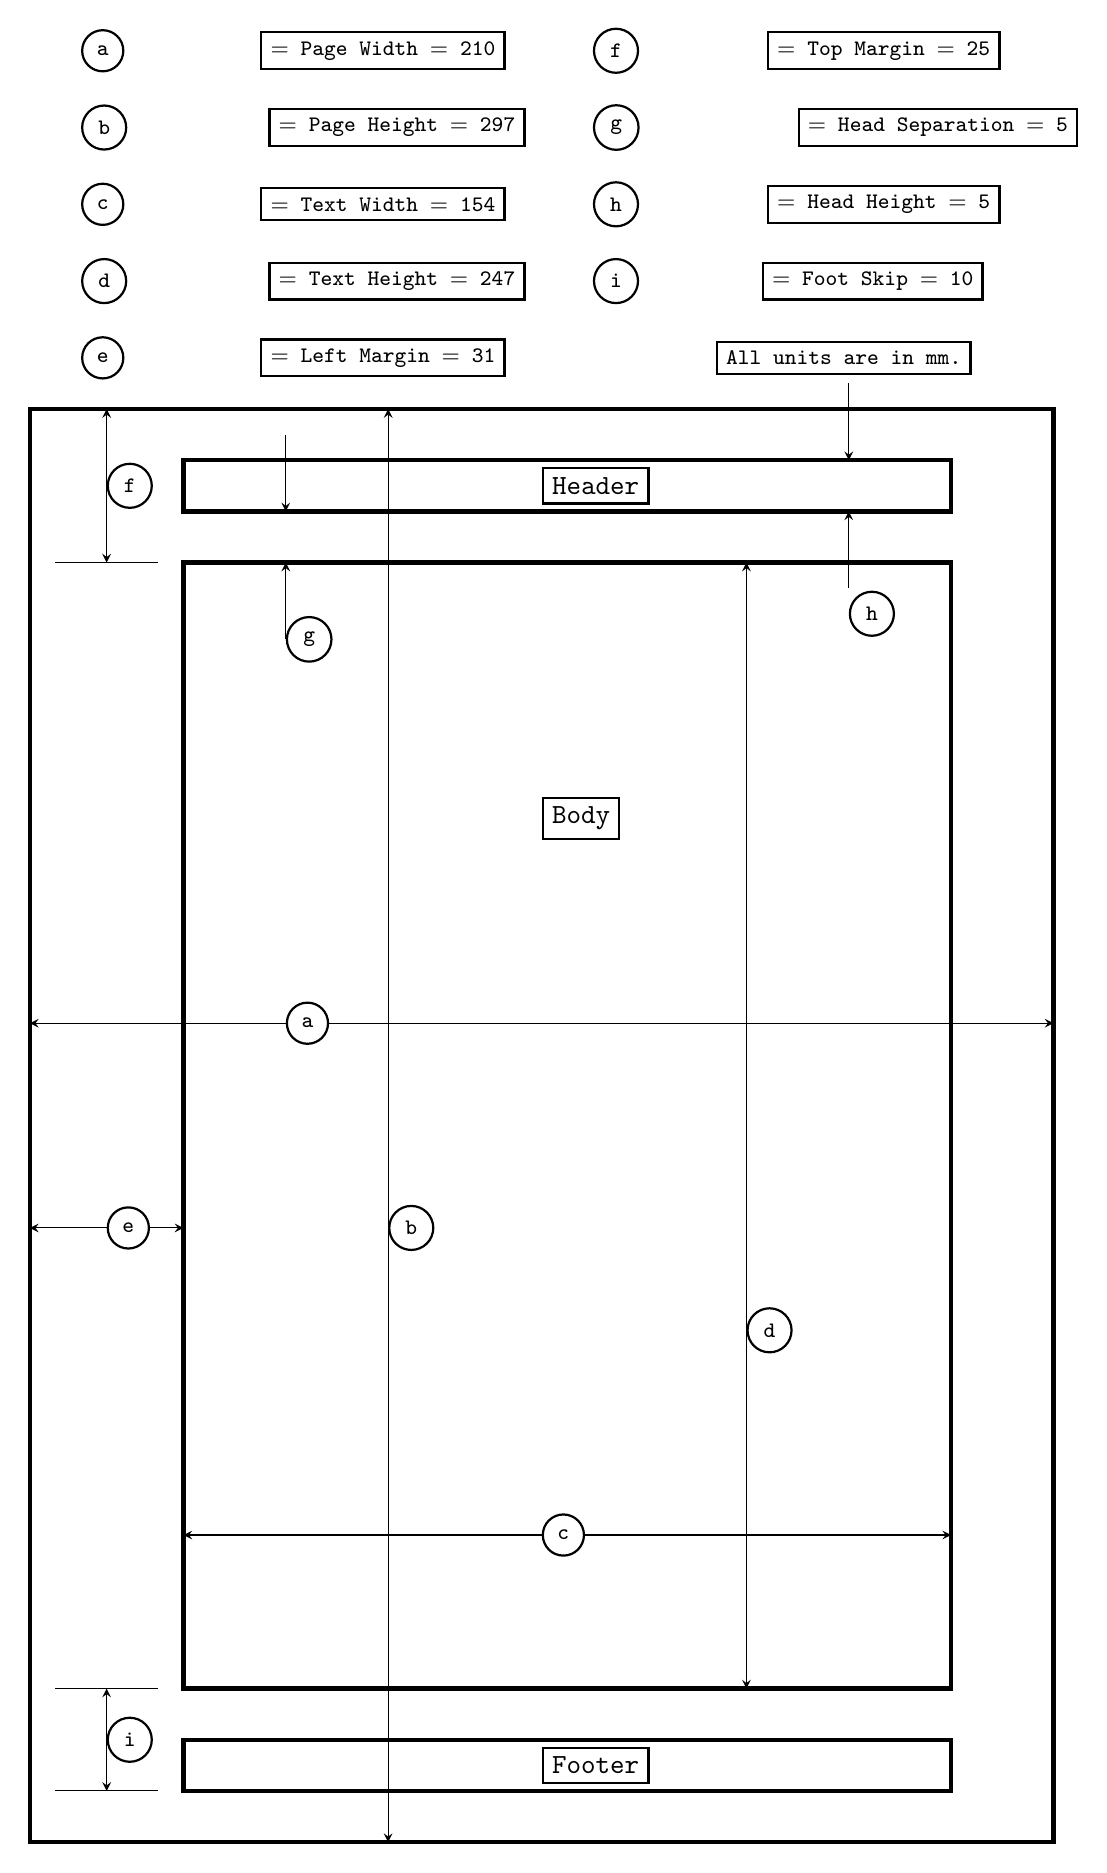
\begin{tikzpicture}[scale=1.3]
%			\draw[step=.5cm,red,very thin] (0,1) grid (12,19);
%			\draw[step=1cm,red,thick] (0,1) grid (12,19);

			\draw[-,ultra thick](1,1)--(11,1)--(11,15)--(1,15)--cycle;
			\draw[-,ultra thick](2.5,2.5)--(10,2.5)--(10,13.5)--(2.5,13.5)--cycle;
			\draw[-,ultra thick](2.5,1.5)--(10,1.5)--(10,2)--(2.5,2)--cycle;
			\draw[-,ultra thick](2.5,14)--(10,14)--(10,14.5)--(2.5,14.5)--cycle;

			\node[font=\normalsize]at(6,11) {{\texttt{Body}}};
			\node[font=\normalsize]at(6,14.25) {{\texttt{Header}}};
			\node[font=\normalsize]at(6,1.75) {{\texttt{Footer}}};

			\draw[<->,>=stealth](1,7)--(2.5,7);
			\node[font=\footnotesize, circle,draw,fill=white]at(1.75,7) {\textbf{\texttt{e}}};
			
			\draw[<->,>=stealth](2.5,4)--(10,4);
			\node[font=\footnotesize, circle,draw,fill=white]at(6,4) {\textbf{\texttt{c}}};
			
			\draw[<->,>=stealth](8,2.5)--(8,13.5);
			\node[font=\footnotesize, circle,draw,fill=white]at(8,6) {\textbf{\texttt{d}}};
			
			\draw[<->,>=stealth](1.75,13.5)--(1.75,15);
			\node[font=\footnotesize, circle,draw,fill=white]at(1.75,14.25) {\textbf{\texttt{f}}};
			\draw[-](1.25,13.5)--(2.25,13.5);
			
			\draw[->,>=stealth](3.5,12.75)--(3.5,13.5);
			\draw[->,>=stealth](3.5,14.75)--(3.5,14);
			\node[font=\footnotesize, circle,draw,fill=white]at(3.5,12.75) {\textbf{\texttt{g}}};
			
			\draw[->,>=stealth](9,13.25)--(9,14);
			\draw[->,>=stealth](9,15.25)--(9,14.5);
			\node[font=\footnotesize, circle,draw,fill=white]at(9,13) {\textbf{\texttt{h}}};
			
			\draw[<->,>=stealth](1.75,1.5)--(1.75,2.5);
			\node[font=\footnotesize, circle,draw,fill=white]at(1.75,2) {\textbf{\texttt{i}}};
			\draw[-](1.25,1.5)--(2.25,1.5);
			\draw[-](1.25,2.5)--(2.25,2.5);
			
			\draw[<->,>=stealth](1,9)--(11,9);
			\node[font=\footnotesize, circle,draw,fill=white]at(3.5,9) {\textbf{\texttt{a}}};
			
			\draw[<->,>=stealth](4.5,1)--(4.5,15);
			\node[font=\footnotesize, circle,draw,fill=white]at(4.5,7) {\textbf{\texttt{b}}};
			
			\node[font=\footnotesize, circle,draw,fill=white]at(1.5,18.5) {\textbf{\texttt{a}}};
			\node[font=\footnotesize, fill=white]at(3.25,18.5) {\texttt{$=$ Page Width $=$ 210 }};
			
			\node[font=\footnotesize, circle,draw,fill=white]at(1.5,17.75) {\textbf{\texttt{b}}};
			\node[font=\footnotesize, fill=white]at(3.33,17.75) {\texttt{$=$ Page Height $=$ 297 }};
			
			\node[font=\footnotesize, circle,draw,fill=white]at(1.5,17) {\textbf{\texttt{c}}};
			\node[font=\footnotesize, fill=white]at(3.25,17) {\texttt{$=$ Text Width $=$ 154}};
			
			\node[font=\footnotesize, circle,draw,fill=white]at(1.5,16.25) {\textbf{\texttt{d}}};
			\node[font=\footnotesize, fill=white]at(3.33,16.25) {\texttt{$=$ Text Height $=$ 247}};
			
			\node[font=\footnotesize, circle,draw,fill=white]at(1.5,15.5) {\textbf{\texttt{e}}};
			\node[font=\footnotesize, fill=white]at(3.25,15.5) {\texttt{$=$ Left Margin $=$ 31}};
			
			\node[font=\footnotesize, circle,draw,fill=white]at(6.5,18.5) {\textbf{\texttt{f}}};
			\node[font=\footnotesize, fill=white]at(8.2,18.5) {\texttt{$=$ Top Margin $=$ 25}};

			\node[font=\footnotesize, circle,draw,fill=white]at(6.5,17.75) {\textbf{\texttt{g}}};
			\node[font=\footnotesize, fill=white]at(8.5,17.75) {\texttt{$=$ Head Separation $=$ 5}};
			
			\node[font=\footnotesize, circle,draw,fill=white]at(6.5,17) {\textbf{\texttt{h}}};
			\node[font=\footnotesize, fill=white]at(8.2,17) {\texttt{$=$ Head Height $=$ 5}};
			
			\node[font=\footnotesize, circle,draw,fill=white]at(6.5,16.25) {\textbf{\texttt{i}}};
			\node[font=\footnotesize, fill=white]at(8.15,16.25) {\texttt{$=$ Foot Skip $=$ 10}};
			
			\node[font=\footnotesize, fill=white]at(7.7,15.5) {\texttt{All units are in mm.}};
	\end{tikzpicture}
\caption{Page size and margin.}
\label{fig-Ch1-Page}
\end{figure}

\item [e.] \textbf{Spacing}\index{spacing}\\
The dissertation should be 1.5-spaced. However, Table of Contents, footnotes, graphs, tables, appendices, list of figures, list of tables, list of algorithms, references, bibliography, and index should be written in single space. Two consecutive paragraphs should be separated by double line spacing.
\item [f.] \textbf{Font}\index{font}\\
The entire dissertation must be written using only a single font including all the texts inside graphs, figures, block diagrams, \textit{etc}. While writing captions of tables and figures, the font size should be decreased by one point. Similarly, the font size of bibliography and index should also be lessened by a point. Students are advised to use the following in the body text~\textemdash
\begin{itemize}
\item[] serif fonts like Times New Roman (TNR) of size 12pt \\
or \\
\textsf{sans-serif fonts like Arial of size 11pt}. 
\end{itemize}
Needless to say that the use of font should be uniform throughout. Headings, Titles \textit{etc.} should use fonts as given below in Table~\ref{tab-fonts}.
{
\linespread{1}
\begin{table}[h]
\centering
\caption{Font sizes to be used in the dissertation}
\begin{tabular}{l C{25mm} C{25mm} c} 
\toprule
{Item} & Arial & {TNR} & {Justification}\\
\midrule\midrule
Main Text & 11 normal & 12 normal & Justified \\
\midrule
Sub-sub Heading & 11 bold & 12 bold & Left \\
\midrule
Sub Heading & 13 bold & 14 bold & Left \\
\midrule
Heading$^{\#}$ & 16 bold & 17 bold & Left \\
\midrule
Chapter Title & 22 bold & 24 bold & Center \\
\midrule
Chapter Number & 16 bold & 17 bold & Left \\
\bottomrule
\multicolumn{4}{l}{$^{\#}$Add serial number with one decimal place.} 
\end{tabular}
\label{tab-fonts}
\end{table}
}
\item [g.] \textbf{Table and Figure}\index{table}\index{figure}\\
All tables, figures, and other such illustrations referenced in the text should be numbered for unique identification. The number format should be $p.q$ with $p$ signifying the chapter number where the illustration appears and $q$ denoting the serial number of that illustration in the chapter $p$. The serial number should be set to 1 at the beginning of a new chapter. A table caption should be placed at the top of the table, and a figure caption should be placed at the bottom of the figure. The caption should follow the unique number $p.q$. The size of the font in the caption of tables and figures should be one less than the text font size. 
\item [h.] \textbf{References}\index{reference}\\
``References'' should be treated as the last chapter and placed at the end of the dissertation. It should not be numbered like other chapters. Texts within the references should have single spacing. The size of the font may be reduced by a point or two. Journal article~\citep{Shannon,Lowe}, Patent~\citep{BulbE,ViBEpatent}, book~\citep{p00e,Vapnik}, conference article~\citep{Toyama,icra}, online resource~\citep{nasa,Kodak}, Ph.D. dissertation~\citep{Sutherland,Dhawan} are usually referred in the text. Some samples of various bibliographic styles are included in this guideline for illustration. You are advised to follow one reference format of any dominant journal of your field.
\end{itemize}

\section{Chapters}\index{chapter}
In the text of the dissertation, each chapter should begin on a fresh page. They should also be designated in the Table of Contents along with other major sections of each chapter. The page numbers listed on the Table of Contents must correlate with the beginning of each section or chapter. All texts should be written with 1.5-spacing. Each chapter should begin with a chapter number in Arabic numerals (font size: Times New Roman 17 points or Arial 16 points, Bold) followed by the chapter title in bold face of size 24 points in Times New Roman font or 22 points in Arial font. %It is preferred to begin a chapter without any section name or number. continuing for a maximum of two paragraphs preferably accommodated within half a page.
\par The first level section should have number of format $a.b$, where the number $a$ is an Arabic number denoting the chapter number and $b$ is also an Arabic number starting from 1 and counting up for each section. For example 3.1, 4.2, or 1.5, \textit{etc}. The section title should follow the section number. Both the title and number should be in the bold face of size 17 points in Times New Roman font or 16 points in Arial font.
\par The second level section should have number of format $a.b.c$, where $c$ is an Arabic number. For example 3.1.1, 4.2.1, or 1.5.2 \textit{etc}. The sub-section title in bold letters should follow the number in bold. The font size should be 14 points Times New Roman or 13 points Arial. Except when it is commonly followed in your field, it is suggested not to give serial number beyond $a.b$ stage, \textit{i.e.} serializing like $a.b.c$ is discouraged.
\par The third level section should have no number. The sub-sub-section title should be in bold letters. The font size should be 12 points Times New Roman or 11 points Arial.
\section{Compilation using \LaTeX}\index{compilation}
The requisite templates\index{template} to assist in formatting\index{formatting} dissertation in \LaTeX~ can be downloaded from \texttt{http://nitris.nitrkl.ac.in} (goto \texttt{Academic -> Dissertation Template}). The folder \texttt{NITRdissertationTemplateV4\_5} contains a number of file and sub folders as shown below in Figure~\ref{fig-Ch1-file}. Fill in the details in \texttt{FrontPages.tex}. Compile your dissertation with the following commands to generate \texttt{DissertationGuidelinesV4\_5.pdf}, or with your preferred integrated development environment (IDE).\\
$>$\texttt{xelatex DissertationGuidelinesV4\_5.tex}\\
$>$\texttt{bibtex DissertationGuidelinesV4\_5}\\
$>$\texttt{xelatex DissertationGuidelinesV4\_5.tex}\\
$>$\texttt{xelatex DissertationGuidelinesV4\_5.tex}\\

\tikzstyle{every node}=[font=\footnotesize,draw=black,thick,anchor=west]
\tikzstyle{selected}=[font=\footnotesize,draw=red,fill=red!30]
\tikzstyle{optional}=[font=\footnotesize,draw=black,fill=gray!50]
\begin{figure}[h]
\centering
\begin{tikzpicture}[%
  grow via three points={one child at (0.5,-.7) and
  two children at (0.5,-0.7) and (0.5,-1.4)},
  edge from parent path={(\tikzparentnode.south) |- (\tikzchildnode.west)},scale=1]
  \node {\texttt{NITRdissertationTemplateV4\_5}}
  	child { node [optional] {\texttt{DissertationGuidelinesV4\_5.tex}}}
  	child { node [optional] {\texttt{FrontPages.tex}}}
  	child { node [optional] {\texttt{NITR.cls}}}
  	child { node [optional] {\texttt{README.txt}}}
  	child { node [optional] {\texttt{DissertationGuidelinesV4\_5.pdf}}}
  	child { node {\texttt{Chap00}}
	  	child { node [optional] {\texttt{Dedication.tex}}}
	  	child { node [optional] {\texttt{Acknowledge.tex}}}
	  	child { node [optional] {\texttt{Abstract.tex}}}
	  	child { node [optional] {\texttt{NITlogo.eps}}}
  	}
    child [missing] {}				
    child [missing] {}				
    child [missing] {}			
    child [missing] {}			
  	child { node {\texttt{Chap01}}
	  	child { node [optional] {\texttt{Guidelines.tex}}}
  	}
    child [missing] {}			
  	child { node {\texttt{Chap02}}
	  	child { node [optional] {\texttt{Unstructured.tex}}}
  	}
    child [missing] {}			
  	child { node {\texttt{Chap03}}
	  	child { node [optional] {\texttt{Conclusion.tex}}}
  	}
    child [missing] {}			
  	child { node {\texttt{SynopsisText}}
	  	child { node [optional] {\texttt{SynopsisText.tex}}}
  	}
    child [missing] {}			
  	child { node {\texttt{Ref}}
	  	child { node [optional] {\texttt{SampleReferences.bib}}}
  		child { node [optional] {\texttt{IEEEtran.bst}}}
  		child { node [optional] {\texttt{asme.bst}}}
	  	child { node [optional] {\texttt{achemso.bst}}}
	  	child { node [optional] {\texttt{bmes.bst}}}
	  	child { node [optional] {\texttt{naturemag.bst}}}
	  	child { node [optional] {\texttt{osajnl.bst}}}
	  	child { node [optional] {\texttt{rsc.bst}}}
	  	child { node [optional] {\texttt{SampleDissemination.tex}}}
  	};
\end{tikzpicture}
\caption{Files and folders in \texttt{NITRdissertationTemplateV4\_5}}
\label{fig-Ch1-file}
\end{figure}